% This is samplepaper.tex, a sample chapter demonstrating the
% LLNCS macro package for Springer Computer Science proceedings;
% Version 2.20 of 2017/10/04
%
\documentclass[runningheads]{llncs}
%
\usepackage{graphicx}
% Used for displaying a sample figure. If possible, figure files should
% be included in EPS format.
%
% If you use the hyperref package, please uncomment the following line
% to display URLs in blue roman font according to Springer's eBook style:
% \renewcommand\UrlFont{\color{blue}\rmfamily}
\usepackage{todonotes}
\begin{document}
%
\title{
}
%
%\titlerunning{Abbreviated paper title}
% If the paper title is too long for the running head, you can set
% an abbreviated paper title here
%
\author{Davide Basile\inst{1}\orcidID{0000-1111-2222-3333} \and
Luca Barbaro\inst{2,3}\orcidID{1111-2222-3333-4444} \and
Valerio Goretti\inst{3}\orcidID{2222--3333-4444-5555}}
%
\authorrunning{F. Author et al.}
% First names are abbreviated in the running head.
% If there are more than two authors, 'et al.' is used.
%
\institute{Sapienza University of Rome}
%
\title{Secure and Scalable Inter-organizational Process Mining through Trusted Execution Environments}
\maketitle

\begin{abstract}
...
\end{abstract}



\section{Introduction}
\label{sec:introduction}
\begin{comment}
\todo[inline]{%
	´CDC: Status corrente secondo me. Abbiamo\ldots
	Un'intro affabile ma che dobbiamo ricalibrare per toglierla dal pantano della TEE e puntare dritto al nostro obiettivo dichiarato e mantenuto, con vista sul potenziale inespresso.\\
	Un motivating scenario che però resta staccato dal resto.\\
	Un related work che però dovrebbe spostarsi sul far capire cosa facciamo di più e di diverso, o di simile ma rivisto.\\
	Una overview eccellente dell'architettura che però non è connessa con l'esempio.\\
	Una overview accurata delle interazioni dei moduli (e quando lo spazio è poco è il caso di fare il merge tra le due cose per risparmiare spazio, come ci dicemmo) -- anche qui senza esempio, dunque capire cosa si fa dove è arduo. Non per me o per te, ma perché conosciamo il lavoro. Chi non lo conosce, non ha assolutamente idea di cosa voglia dire fare il merge degli eventi da tracce provienienti da actor diversi rimettendoli in ordine così da preservare integrità temporale, per esempio.\\
	Una discussion/evaluation ben congegnata in cui però manca la parte quantitativa e la qualitativa è ancora da dettagliare.\\
	Una conclusione.%
}
\end{comment}
In today's business landscape, organizations constantly seek ways to enhance operational efficiency, increase performance, and gain valuable insights to improve their processes. Process mining offers techniques to discover, monitor, and improve business processes by extracting knowledge from chronological records known as \textit{event logs} \cite{van2012process}. Organizations record in these ledgers events referring to activities and interactions occurring within a business process. The vast majority of process mining contributions consider \textit{intra-organizational} settings, in which business processes are executed inside individual organizations. However, organizations increasingly recognize the value of collaboration and synergy in achieving operational excellence. \textit{Inter-organizational} business processes involve several independent organizations cooperating to achieve a shared objective \cite{van2011intra}. Despite the advantages of transparency, performance optimization, and benchmarking that companies can gain from such practices, inter-organizational process mining raises challenges that make it still hardly applicable. The major issue concerns confidentiality. Companies are reluctant to outsource to their partners inside information that is required to execute process mining algorithms. Indeed, the sharing of sensitive operational data across organizational boundaries introduces concerns about data privacy, security, and compliance with regulations. \textit{Trusted Execution Environments} (TEEs) can serve as fundamental enablers to balance the need for insights with the imperative to protect sensitive information in inter-organizational settings. TEEs offer secure contexts that guarantee code integrity and data confidentiality in external devices. \textit{Trusted applications} are tamper-proof software objects running in these environments. 

In this paper, we propose the CONFINE framework for inter-organizational process mining. It resorts to trusted applications to preserve the secrecy and integrity of shared data. To pursue this aim, we design a decentralized software architecture for a four-staged protocol: (i) The initial exchange of preliminary metadata, (ii) The attestation of the miner entity, (iii) the secure transmission of encrypted data amid multiple parties, (iiii) The privacy-preserving merge of the shared information segments followed by the isolated and verifiable computation of process discovery algorithms on joined data.
We evaluate our proof-of-concept implementation against synthetic and real-world-based data with a convergence test and memory effectiveness assessment.

The remainder of the paper is structured as follows: \cref{sec:background} provides an overview of related work inherent to the theme of inter-organizational process mining. In \cref{sec:motivating}, we introduce a use case example that considers a healthcare scenario. The CONFINE architecture is presented in \cref{sec:design}. Following on from this, we instantiate the addressed design principles in \cref{sec:realization}, focusing on the employed technologies, communication protocol, and implementation. In \cref{sec:evaluation}, we discuss our solution. Finally, we conclude and present directions for future work in \cref{sec:conclusion}.

\section{Related Work}
\todo[inline]{It can be reduced. EDIT: Already reduced. MISSING: what do we do similarly to and what do we do differently from / improve on the cited papers? A comparison is offered only with the work of M{\"u}ller et al.}
\label{sec:background}
%First inspiration work
% Inter-organizational and process mining
\begin{comment}
The work of M{\"u}ller et al.~\cite{muller2021process} is the first contribution that considers TEEs in combination with blockchain technologies for process mining purposes. This research proposes a conceptual architecture in which process mining algorithms are executed inside centralized third-party services. Inspired by this preliminary contribution, we design a decentralized approach context where each organization can run process mining algorithms without involving external stakeholders.
The literature proposes several studies that consider process mining techniques in inter-organizational environments. Van Der Aalst~\cite{van2011intra} shows that inter-organizational processes can be divided according to different dimensions making identifiable challenges of inter-organizational process extractions. Elkoumy et al.~\cite{elkoumy2020shareprom} propose a tool that allows independent parts of an organization to perform process mining operations by revealing only the result. This tool is called Shareprom and exploits the features of secure multi-party computation (MPC). Engel et al.~\cite{engel2016analyzing} present EDImine Framework, which allows to apply process mining operations for inter-organizational processes supported by the EDI standard\footnote{https://edicomgroup.com/learning-center/edi/standards} and evaluate their performance using business information.
Elkoumy et al.~\cite{elkoumy2020secure} propose an MPC-based architecture that aims to perform process mining operations without sharing their data or trusting third parties.
% inter-organizational and merge log
Applying process mining techniques in intra-organizational contexts requires merging the event logs of the organizations participating in the process. The literature offers several studies in this area. For instance, Hernandez-Resendiz et al.~\cite{hernandez2021merging} present a methodology for merging logs at the trace and activity level using rules and methods to discover the process. Claes et al.~\cite{claes2014merging} provide techniques for performing merge operations in inter-organizational environments. This paper indicates rules for merging data in order to perform process mining algorithms.
%data exchange 
The state of the art provides some studies that investigate issues and possible solutions regarding data exchange, more specifically in an business collaboration context. EDI standards enable the communication of business documents. Among these standards, the notion of process is not explicitly specified. This inhibits organizations from applying Business Process Management (BPM) methods in business collaboration environments. Engel et al.\cite{engel2011process} extended process mining techniques by discovering interaction sequences between business partners based on EDI exchanged documents. Lo et al.\cite{lo2020flexible} have provided and developed a framework for data exchange designed even in intra-organizational situations. This framework is based on blockchain and decentralized public key infrastructure technologies, which ensure scalability, reliability, data security, and data privacy.
% Use of data from other organizations(or person) integrity ecc ecc (LOCAL)
Additionally, there are several papers that propose solutions for the correct sharing and use of data by third parties. Xie et al.\cite{XIE2023321} propose an architecture for the internet of things based on TEE and blockchain. The proposed architecture aims to solve data and identity security problems in the process of data sharing. Basile et al.~\cite{Basile_Blockchain_based_resource_governance_for_decentralized_web_environments} in their study created a framework called ReGov that allows the exchange of sensitive information in a decentralized web context, ensuring usage control-based data access and usage. In order to control the consumer's device ReGov uses TEE that allows storage and utilization management of retrieved resources. Hussain et al.\cite{hussain2021sharing} present a tool for privacy protection and data management among multiple collaborating companies. This tool allows data encryption to be configured according to the privacy obligations dictated by the context of a system's use. 

\end{comment}

\todo[inline]{Our work revolves around the following areas: 1, 2 and 3. Next, we position our contribution against the existing body of literature.}

The work of M{\"u}ller et al.~\cite{muller2021process} is the first contribution that considers TEEs in combination with %blockchain technologies for process mining purposes.
process mining techniques.
% \todo{When do we use blockchain in this paper? If we do not use it, then we should make clear why we do not. Isn't it also the first paper that uses TEE for process mining? If it is, then we omit this blockchain thing and take it back for future work perhaps or as an additional detail.}
This research proposes a conceptual architecture in which process mining algorithms are executed inside centralized third-party services. Inspired by this preliminary contribution, we design a decentralized approach context where each organization can run process mining algorithms without involving external stakeholders. The theme of inter-organizational process mining is discussed in the literature from different perspectives. Van der Aalst~\cite{van2011intra} highlights the challenges of inter-organizational process extraction through a categorization. Elkoumy et al.~\cite{elkoumy2020shareprom} introduce Shareprom, a secure tool for inter-organizational process mining based on secure multi-party computation (MPC). Engel et al.~\cite{engel2016analyzing} present the EDImine Framework, which applies process mining to inter-organizational processes using the EDI standard. In inter-organizational contexts, merging event logs from different organizations is essential. Hernandez-Resendiz et al.~\cite{hernandez2021merging} propose a methodology for log merging, while Claes et al.~\cite{claes2014merging} provide techniques for merging data to support process mining algorithms. Data exchange in business collaboration environments has already been explored in various works. Engel et al.~\cite{engel2011process} extend process mining by analyzing interaction sequences based on EDI documents. Lo et al.~\cite{lo2020flexible} present a blockchain-based framework for secure data exchange, even within inter-organizational scenarios. Lastly, there are solutions for secure data sharing with third parties. Xie et al.~\cite{XIE2023321} propose an IoT architecture using TEE and blockchain. Basile et al.~\cite{Basile_Blockchain_based_resource_governance_for_decentralized_web_environments} introduce ReGov for controlled data utilization in decentralized web contexts.% Hussain et al.~\cite{hussain2021sharing} offers a tool for privacy protection and data management in collaborative settings, allowing data encryption to align with privacy requirements.
In the fast-evolving landscape of healthcare, seamless collaboration between multiple organizations is essential to ensure the highest standard of patient care. We delve into the application of Trusted Execution Environment (TEE) to facilitate the secure exchange of event logs between three pivotal actors: an esteemed hospital, a specialized clinic, and a leading pharmaceutical company. This innovative approach fosters a robust and trustworthy ecosystem where sensitive patient data can be shared securely, promoting seamless collaboration for the betterment of patient outcomes.


In this section, we present the high-level architecture of our CONFINE framework. We consider the main functionalities of each component, avoiding details on the employed technologies discussed in the next sections. After introducing the architecture, we focus on the \Compo{Secure Miner}, a core component of our contribution.

\subsection{CONFINE architecture at large}
Our architecture involves different organizational ecosystems characterized by one or more machines. An organization may take at least one of the following roles: 
\begin{inparadesc}
\item[provisioning] if it delivers local event logs to be collaboratively mined;
\item[mining] if it applies process mining algorithms using event logs retrieved from provisioners.
\end{inparadesc}
% Provisioners collaborate to achieve common objectives and compose inter-organizational business processes whose event logs are scattered across multiple places. 
% Provisioners produce event logs, recording the operations executed to complete their part in the inter-organizational business process.
In \cref{fig:architecture_diagram}, we propose the high-level schematization of our solution.
In our solution, every organization hosts one or more \Compo{Node}s. Depending on the played role, \Compo{Node}s come endowed with a \Compo{Provisioner} or a \Compo{Secure Miner} component, or both. The \Compo{Provisioner} component consists of the following two main sub-components. The \begin{inparadesc}
\item[\Compo{Log Recorder}] registers the events taking place in the organizations' systems. The
\item[\Compo{Log Provider}] delivers on-demand data to mining players.
\end{inparadesc}
The \Actor{Hospital} (as well the other parties in our running example) records Alice and Bob's traces using the \Compo{Log Recorder}. The \Compo{Log Recorder} is queried by the \Compo{Log Provider} for event logs to be made available for mining. The latter controls access to local event logs by authenticating data requests by miners and rejecting those that come from unauthorized parties.
In our motivating scenario, the \Actor{Specialized clinic}, \Actor{Pharmaceutical company}, and the \Actor{Hospital} leverage \Compo{Log Provider}s to authenticate the miner party before sending their logs.  The \Compo{Secure Miner} component
% \Compo{Log Provider}s reject demands from unauthorized parties and only permit \texttt{Secure Miners} to use the data. 
% The \Compo{Secure Miner} 
shelters external event logs inside a protected environment to preserve data confidentiality and integrity.
Notice that \Compo{Log Provider}s accept requests issued solely by \Compo{Secure Miner}s. 
Next, we provide an in-depth focus on the latter.
% We provide an in-depth focus on this key component in the following.
\begin{comment}
\begin{figure}[t]
	\centering
	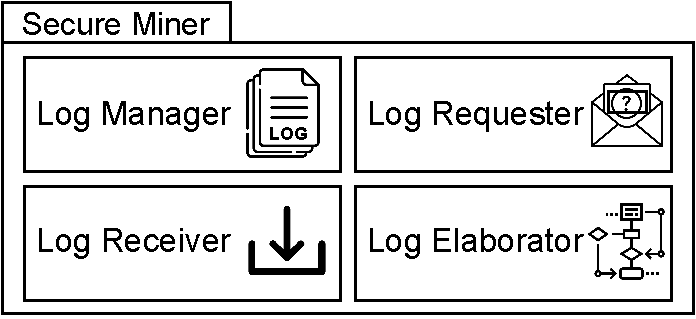
\includegraphics[width=0.5\linewidth]{content/figures/secureminersad.pdf}
	\caption{Subcomponents of the Secure Miner.}
	\label{fig:trusted_miner}
\end{figure}
\end{comment}

\begin{figure}[t]
	\centering
	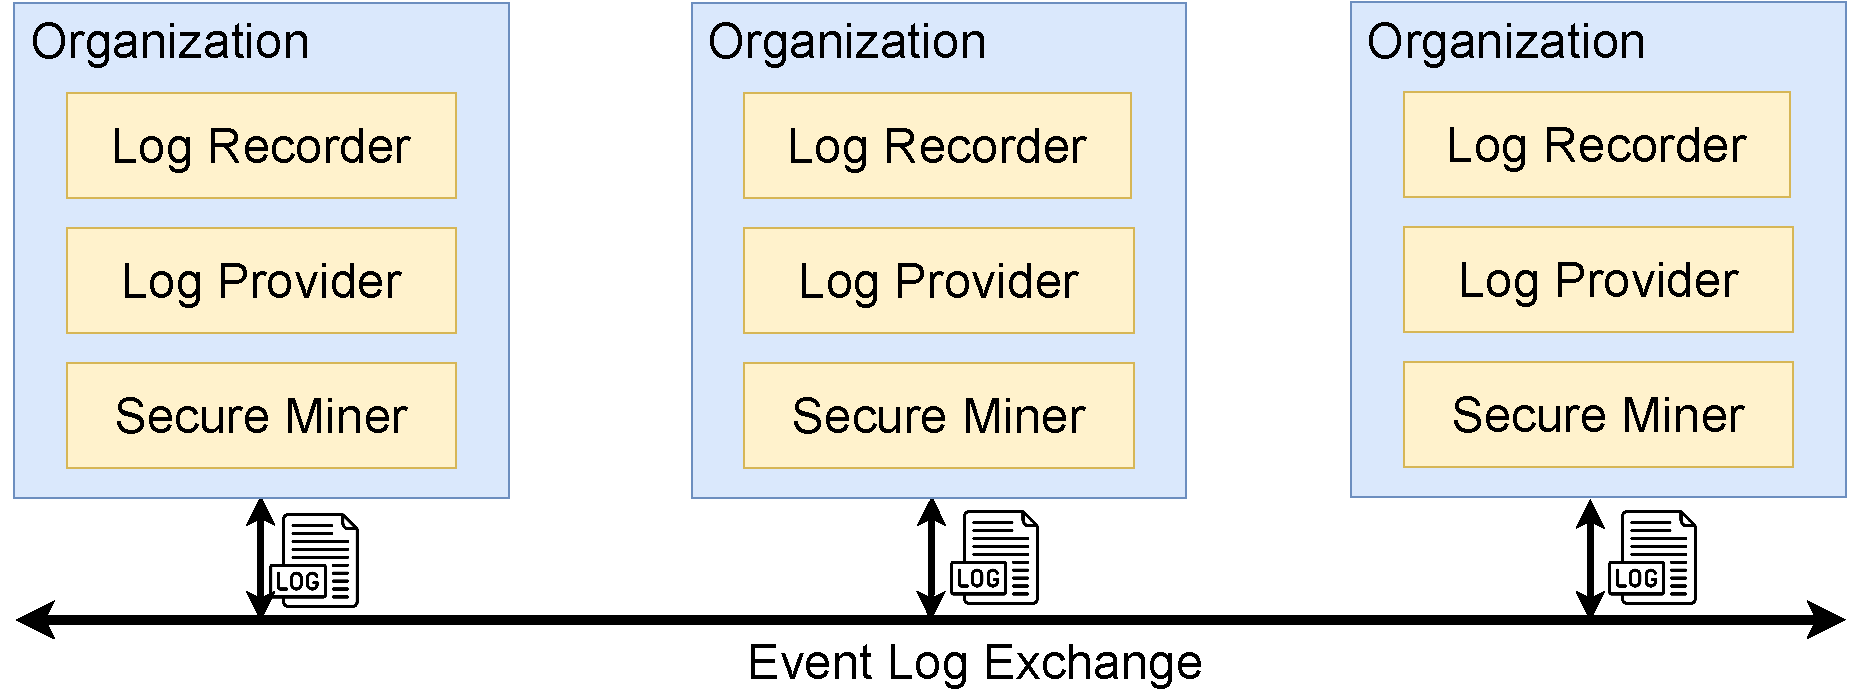
\includegraphics[width=0.79\linewidth]{content/figures/architecturediagram.pdf}
	\caption{High-level architectural overview.}
	\label{fig:architecture_diagram}
\end{figure}

\begin{wrapfigure}[9]{r}{0.4\textwidth}
	\vspace{-2em}
	\centering
	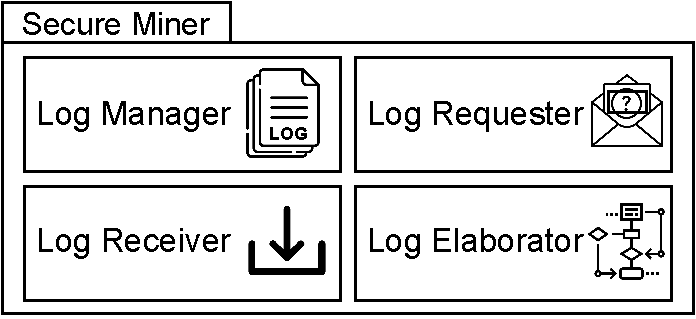
\includegraphics[width=1\textwidth]{content/figures/secureminersad.pdf}
	\caption[A gull]{Sub-components of the \\Secure Miner.}
	\label{fig:trusted_miner}
	\vspace{-6pt}
\end{wrapfigure} 
\subsection{Secure Miner}
The primary objective of the \Compo{Secure Miner} is to allow miners to securely execute process mining algorithms using event logs retrieved from provisioners such as the \Actor{Specialized clinic}, \Actor{Pharmaceutical company}, and the \Actor{Hospital} of our running example. \Compo{Secure Miner}s are isolated components that guarantee data inalterability and confidentiality. In \cref{fig:trusted_miner}, we show a schematization of the \Compo{Secure Miner}, which consists of four sub-components:
\begin{inparaenum}[\itshape(i)\upshape]
    \item The \Compo{Log Requester};
    \item The \Compo{Log Receiver};
    \item The \Compo{Log Manager}; 
    \item The \Compo{Log Elaborator}.
\end{inparaenum}
%Event logs belonging to provisioners are locked in the \Compo{Secure Miner}.
%We handle  data via the 
The \Compo{Log Requester} and the \Compo{Log Receiver} are the sub-components that we employ during the event log retrieval. \Compo{Log Requester}s send authenticable data requests to the \Compo{Log Provider} component of provisioners. The \Compo{Log Receiver} collects event logs sent by \texttt{Log Providers} and entrusts them to the \Compo{Log Manager}, securing them from accesses that are external to the \Compo{Secure Miner}.
Miners of our motivating scenario, such as the \Actor{University} and the \Actor{National Institute of Statistics}, employ these three components to retrieve and store Alice and Bob's data. The \Compo{Log Elaborator} merges the event data locked in the \Compo{Secure Miner} to have a global view of the inter-organizational process comprehensive of activities executed by each involved party. Thereupon, it executes process mining algorithms in a protected environment, inaccessible from the outside computation environment.
In our motivating scenario, the \Compo{Log Elaborator} combines the traces of Alice (i.e., $T^H_{312}$, $T^S_{312}$, and $T^C_{312}$) and Bob (i.e, $T^H_{711}$, $T^S_{711}$, and $T^C_{711}$), generates the chronologically sorted traces $T_{312}$ and $T_{711}$, and feeds them into the mining algorithms (see the bottom-right quadrant of \cref{tab:trace}).




\section{Realization}
\label{sec:implementation}
%Focus generale sulle tecnologie utilizzate
In this section we outline the technical aspects concerning the realization of our framework. Therefore we first present the enabler technologies through which we instantiate the design principles presented in \cref{sec:design}. After that, we discuss the interaction workflow between the instantiated technologies. Finally, we show the implementation details.
\begin{figure}[t]
\centering
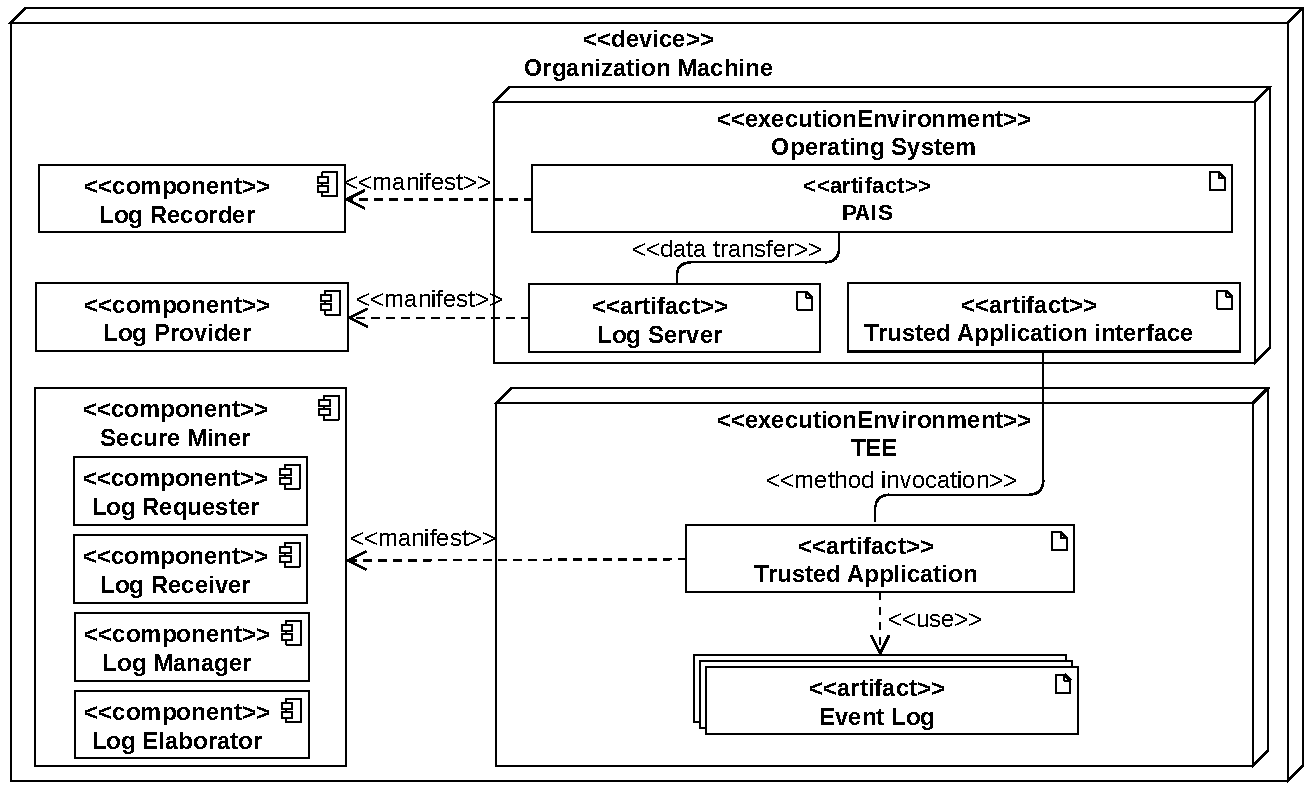
\includegraphics[width=10 cm]{content/figures/deployment_diagram.pdf}
\caption{UML deployment diagram.}
\label{fig:deployment_diagram}
\end{figure}
\subsection{Deployment}
As follow, we bridge the gap between high-level system architecture and its practical realization. \cref{fig:deployment_diagram} depicts a \textit{UML deployment diagram} \cite{koch2002expressive} that aims to help with understanding the instantiated infrastrucuture. 

The \texttt{Organization Machine} represent the physical computation \textit{device} embracing the software and hardware entities of the company. The \texttt{Log Recorder}, the \texttt{Log Provider} and \texttt{Secure Miner} are included in the \texttt{Organization Machine} as abstract \textit{components} . These logical elements incorporate the core functionalities already discussed in \cref{sec:design}. The \texttt{Organization Machine} is characterized by two \textit{execution environment}s namely the \texttt{Operative System} and the \texttt{Trusted Execution Environment}.

Software entities that we expose to the users of the \texttt{Organization Machine} run inside the \texttt{Operative System}. We mainfest the functionalities offered by the \texttt{Log Recorder} in the \texttt{Process Aware Information System}  \cite{Dumas.etal/2018:FundamentalsofBPM}. These systems help users to handle business processes including accounting and resource management. In our solution, the \texttt{Process-Aware Information System} provides the \texttt{Log Server} access to event logs. \texttt{Log Servers} are web services which processes remote data request and provides event log to miners. We build this entities upon existing web standards such as HTTP, FTP and Goopher.

\texttt{Trusted Execution Environment}s are the core technologies of our solution. It creates a separated context from the normal \texttt{Operating System} to protect code and data through hardware-based security features in a reserved zone of the \texttt{Organization Machine}'s CPU. We leverage the security guarantees offered by this techonologies to instantiate a \texttt{Trusted Application} to fulfill the functionalities of the \texttt{Secure Miner} and its subcomponents. The \texttt{Trusted Application} collect the logic generate verifiable data request, receive event external logs, store them in the \texttt{Trusted Execution Environment}, and apply process mining algorithms. Procedures executed by the \texttt{Trusted Application} are tamperproof. The \texttt{Trusted Execution Environment} ensures that the code of the \texttt{Trusted Application} executed within it is protected from unauthorized accesses and malicious manipulations. We employ the isolated context of \texttt{Trusted Execution Environment} to store \texttt{Event Log}s of partner orgnizations inside the miner machine. The \texttt{Trusted Execution environment} provide mechanism to protect this sensitive information withoutg exposing it to the \texttt{Operative System}. The \texttt{Trusted Application} is the only entity that can access the \texttt{Event Log}s and feed them to process mining algorithms. Users can communicate with the \texttt{Trusted Application} via the \texttt{Trusted Application Interface}. The \texttt{Trusted Application} offer secure methods to safely receive information from  the \texttt{Operative System} and present the outputs of the computation. These methods are invoked by the \texttt{Trusted Application Interface} and instantiate the only communication channel to the \texttt{Trusted Application}.
%What the secure miner can do
%-TEEs ensure that the code and data executed within the environment are protected from unauthorized access
%TEEs provide mechanisms to protect sensitive data stored within the environment. Encryption and decryption operations can be performed securely without exposing the data to the less secure parts of the system.
%


%The \texttt{PAIS Interface} collects the logic to interact with the Process-aware Information Sytem (\texttt{PAIS}) of the \texttt{Organization}. \texttt{PAIS} systems help \texttt{Organization}s to handle business processes including accounting and resource management. The maintenance of event logs is the core tasks performed by these systems~\cite{Dumas.etal/2018:FundamentalsofBPM}. In our architecture, we generalize the interaction with \texttt{PAIS}s through the \texttt{PAIS Interface}. The \texttt{PAIS Interface} is queried by the local \texttt{Log Provider} for event logs to be fed into \texttt{Secure Miner}s.
\begin{figure}[t]
\centering
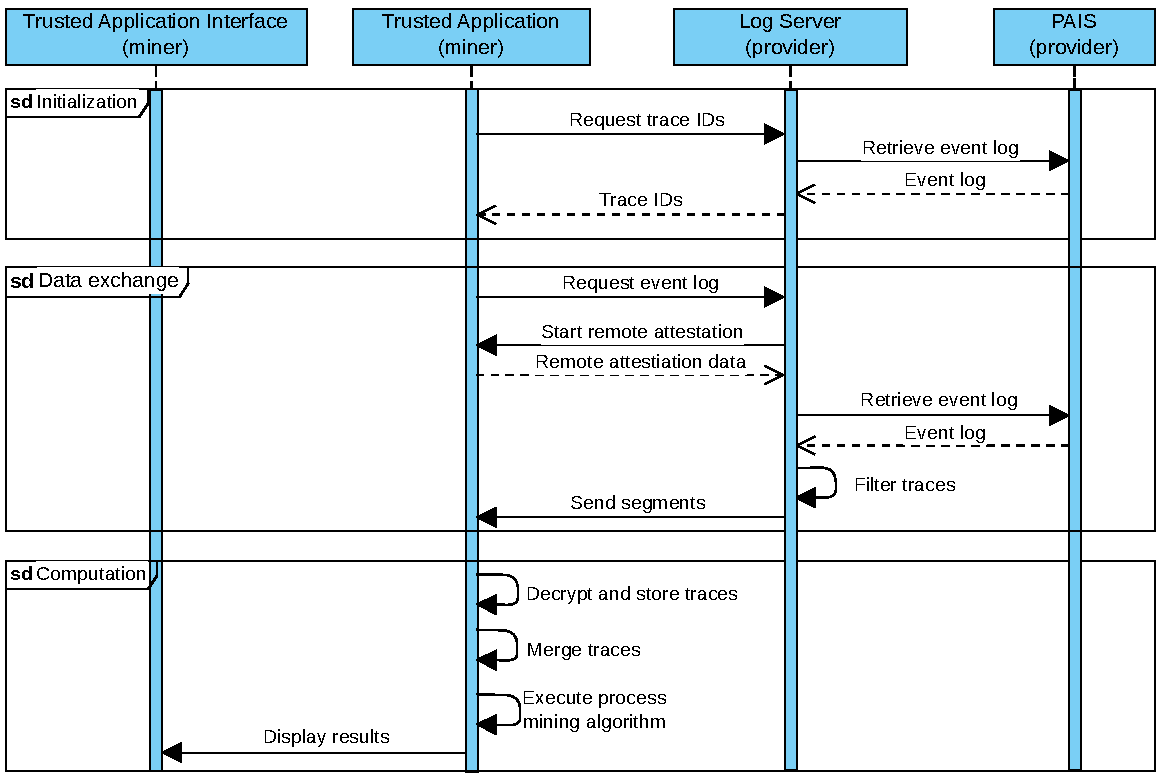
\includegraphics[width=10.5cm]{content/figures/sequence_diagram.pdf}
\caption{UML sequence diagram.}
\label{fig:sequence_diagram}
\end{figure}
\subsection{Workflow}
As follow, we analyze the data flows and interactions among the introduced technologies. We separate the workflow into subsequent processes namely \textit{initialization}, \textit{data exchange} and \textit{computation}.
The parties involved in the workflow are a miner (i.e., an organization that execute process mining algorithms) and one or more providers (i.e., partner organizations that serve their event logs). %We distinguish three different phases of the process namely the \textit{initialization}, the \textit{data exchange}, and the \textit{computation}.

\textbf{Initialization.} In the initialization, the miner's \texttt{Trusted Application} requests preliminary information from the providers' \texttt{Log Server} concerning the event logs of an inter-organizational business process. After authenticating the sender, the involved \texttt{Log Server}s retrieve the local event log from the \texttt{Process-Aware Information System} and respond the miner by providing the list of trace IDs in the event log. Hence, the \texttt{Trusted Application} collect the responses and store them in the \texttt{Trusted Execution Environment}.

\textbf{Data exchange.} Once recorded the preliminary information, the miner starts the data exchange. Therfore, its \texttt{Trusted Application} sends data requests to the \texttt{Log Servers}. The requests include as parameters the list of trace ids and the segment size. Subsequently, the \texttt{Log Server}s starts the \textit{remote attestation} procedure thanks to which they can verify that the sender of the log request: is a \texttt{Trusted Application} running inside a \texttt{Trusted Execution Environment}; comes from a partner organization. This operation involve the exchange of additional messages between the \texttt{Log Server} and the \texttt{Trusted Application}. If the procedure is successful, the identity of the miner is verified %and its public key determined.
Subsequently, the \texttt{Log Servers} retrieve the local event log and filter its traces according to the trace IDs sent by the \texttt{Trusted Application}. Filtered event logs are splitted in several segments containg traces whose dimension does not exceed the segment size parameter. \texttt{Log Servers} encrypts the segments and send each of them to the \texttt{Trusted Application}. The \texttt{Trusted Application} decrypt the received segments, extract the traces and store them in \texttt{Event Log}s inside the \texttt{Trusted Execution Environment}.

\textbf{Computation.} To start a computation routine, the \texttt{Trusted Application} needs all partner organizations to have delivered traces having the same ID. When this occurs, the \texttt{Trusted Application} merges external traces with the owned one. Assebled traces are used as parameter of process mining algorithms executed by the \texttt{Trusted Application} that presents the result of the computation to the users via the \texttt{Trusted Application Interface}.
\subsection{Implementation}
In this section, we describe the implementation of our paper. The implementation proposed integrates a trusted application running in a
trusted execution environment and some event logs generated to address the solution proposed in the motivating scenario. The code is available at the following address: \url{https://github.com/dave0909/TEExProcessMining/}

%\subsubsection{Event Log Generation}
%Technologies Used
%Summary of the log generation process
In order to generate the logs for the execution of the trusted application, a process model was created based on BPMN notation\footnote{https://www.bpmn.org}. Subsequently, the model was imported into the BIMP\footnote{https://bimp.cs.ut.ee} software, which made it possible to generate the synthetic event logs. The number of log traces generated through BIMP aligns with other works in the state of the art; the generation software was set to 1000 traces. Following the generation, the synthetic event log relating to the process model was filtered via ProM \footnote{https://promtools.org}. We were able to filter the logs based on attribute values, which allowed us to filter the synthetic log according to the resource involved in the activities. Referring to the motivating scenario, the resources involved are the hospital, the specialised clinic, and the pharmaceutical company. In this way, we created three separate event logs from the initial event log, which were used to exchange data between the organisations.

%{Trusted Miner and Log Provider}
%TEE technology used
%Language used to program in TEE
%Algorithm implemented
%Intermediate representations (PNML, Petrinet, etc.)
Referring to the trusted execution environment, we used a framework called EGo\footnote{https://www.edgeless.systems/products/ego/}, which makes it possible to develop trusted applications programmed in GO\footnote{https://go.dev}. We developed the Trusted Application (TA) within the TEE with the same language. Within the TA there is the "Secure Miner" module, which allows logs from other organisations to be requested, managed, and processed. Log processing is made possible by the implementation of the "Heuristc Miner" process mining algorithm\ref{weijters2006process}, which takes the log traces as input and performs a discovery operation.
The output of the algorithm is a PNML\footnote{https://www.pnml.org}(Petri Net Markup Language) which allows the representation of Petri nets that graphically illustrate the model calculated by the algorithm. 
%The output of the algorithm is a file with the extension '.pnml'. PNML\footnote{https://www.pnml.org}(Petri Net Markup Language) is a markup language that allows the representation of Petri nets that graphically illustrate the model calculated by the algorithm. 
In order to generate the graphic image of the Petri net, the WoPed\footnote{https://woped.dhbw-karlsruhe.de} software was used, which takes as input a PNML file and provides the graphic representation of the Petri net. 

%Log provider language
Another fundamental module within the TA is that of the Log Provider. This part of the TA is also written in Go and is listening on one of the ports set up by the organisation owning the application. It accepts requests made by other organisations and forwards its log. 


\section{Evaluation}
\subsection{Discussion}
\subsubsection{Privacy}
\subsubsection{Security}
\subsubsection{Integreatebility}
\subsection{Convergence Study}
\subsubsection{Settings}
\subsubsection{Results}
\section{Conclusion and Future Work}
\label{sec:conclusion}
Confidentiality is of paramount importance in inter-organizational process mining due to the transmission of sensitive data across organizational boundaries. Our research investigates a secrecy-preserving approach that enables organizations to employ process mining techniques with event logs from multiple organizations while ensuring the protection of privacy and confidentiality. Our solution still has room for improvement. We operate under the assumption of fair conduct by data provisioners and do not account for the presence of injected or maliciously manipulated event logs. In addition, we do not handle TEE crashes and suppose that miners and providers exchange messages in perfect communication channels where no loss, no snap, and no bit corruption occours. Additionally, our approach relies on certain assumptions about event log data, including the existence of a universal clock for event timestamps, which may not be realistic in situations where organizations are not perfectly synchronized. To address this challenge, we intend to explore a solution based on Network Time Protocols (NTP). Our future work encompasses the development of a formalized interaction protocol governing the communication between data provisioners and miners. The presented solution embraces model process mining techniques in a general way. However, we believe that the presented approach is particularly compatible with declarative model representations. Therefore, trusted applications could compute and store the entire set of rules representing a business process, and users may interact with them via trusted queries. Finally, in our implementation, we have focused on process discovery tasks. However, our approach has the potential to seamlessly cover a wider array of process mining functionalities such as \textit{conformance checking}, and \textit{performance analysis} techniques. Implementing them and show their integrability with our approach paves the path for future work. 
%\todo{CDC: The bibliography entries are too rich. Look at \cite{engel2011process}. Do we really care that the conference was in Toulouse? And look at \cite{koch2002expressive}: the acronym is enough for the conference name. Also, the volume number is useless if we do not have the series (anyway, we could not care less about either of the two). We have already gone through this, so we should shorten the entries as we know.}

\begin{comment}
Limitations:
\begin{itemize}
    \item Both producer and consumer act fairly (so we do not expect to have injected data) ok
    \item We do not manage TEE crashes
    \item We assume a perfect communication channel (no loss, no snap, no corrupted bits)
    \item Universal clock for event timestamps (cite Event log cleaning for business process analytics by Andreas Solti)
\end{itemize} 
Future Work:
\begin{itemize}
    \item Declarative models adaptation ok
    \item Output inside the TEE, interactions through trusted applications
    \item Real-world event log data ok
    \item Usage policies integration ok
    \item Formal interaction protocol ok
    \item Threat model ok
    \item Security evaluation ok
\end{itemize}
\end{comment}
%future work, quali segment portano al risultato attuale e farlo per ogni risultato intermedio -call valerio claudio 9-06-23


%%%%%%%%%%%%%%%%%%%%%%%%%%%%%%%%%%%%%%%%%%%%%
% Biblography
%%%%%%%%%%%%%%%%%%%%%%%%%%%%%%%%%%%%%%%%%%%%%
\bibliographystyle{ieeetr}
\bibliography{main}


\end{document}
